\chapter{Conclusion}

In the initial state, there was no sophisticated visualization for data from the ATLAS-TPX network. This work has proposed a universal storage system, capable of holding data captured by 15 detectors in the ROOT file format. It has also defined an auxiliary database built atop SQL, which has achieved the acceleration of the most common queries through various performance optimization techniques. An interactive web visualization UI has been designed and implemented along with a server-side component to transcode TPX data into JSTP, a proprietary data format defined to efficiently encode frames for network transfers. The architecture of the server implementation allows multiple users to operate the system simultaneously by the use of multi-threading.

At the time of writing this work, the web visualization UI is available\footnote{\url{http://atlastpx.utef.cvut.cz}} online. It is capable of displaying frames from single as well as multiple TPX detectors simultaneously. However, apart from plotting charts and calculating various statistics, it also allows its users to interact with the displayed content by applying magnification, setting arbitrary predicates and integrating over consecutive frames. For that reason, it has various applications in data analysis and visualization, and can be used in other experiments involving Timepix detectors.

\begin{figure}[t]
\begin{center}
	\begin{subfigure}{\textwidth}
	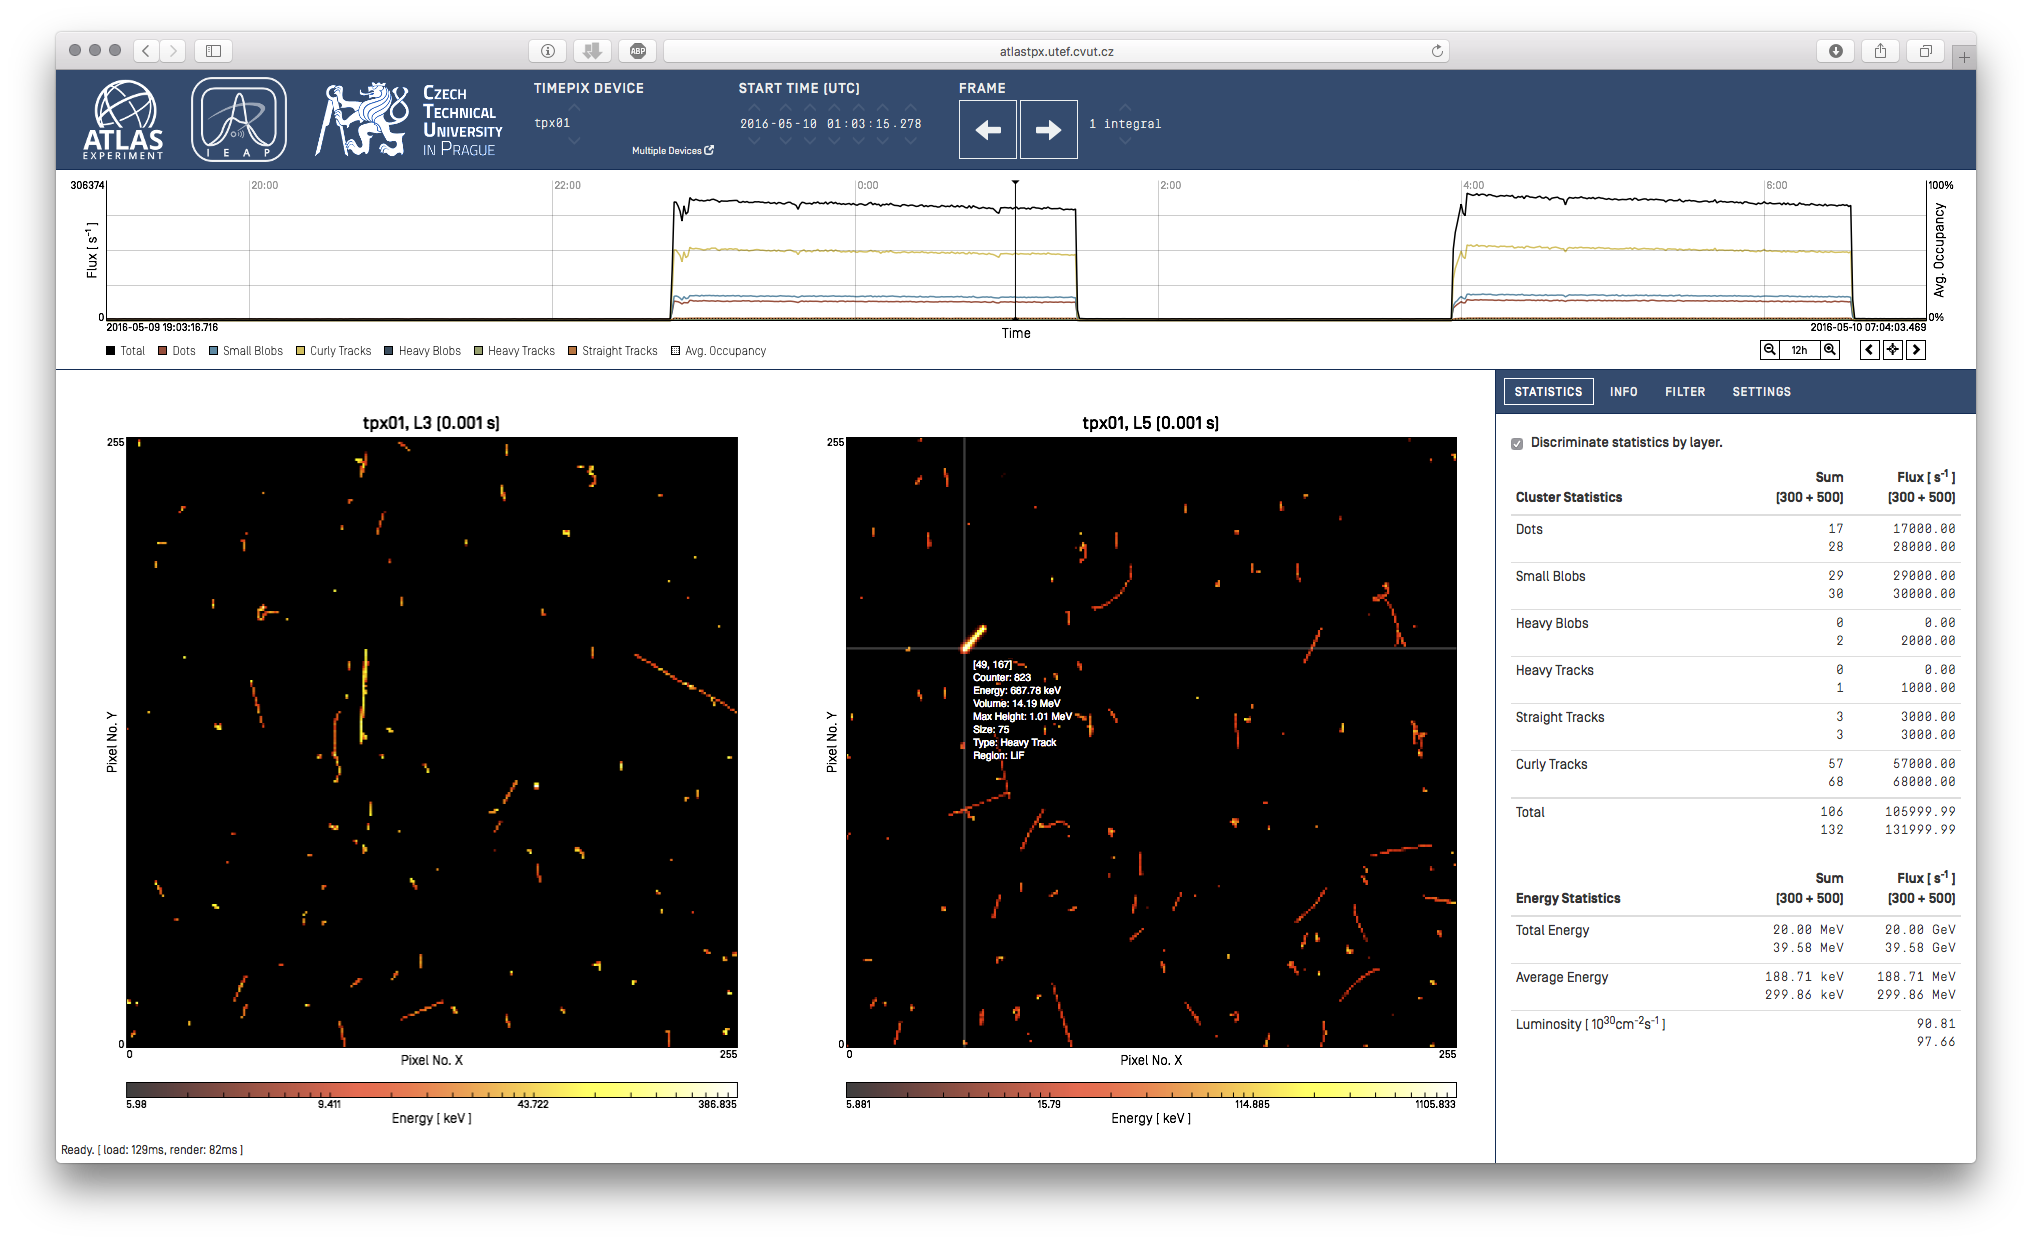
\includegraphics[width=\textwidth]{figures/screen-tpx01-crosshair}
	\caption{Visualization in regular operation mode.}
	\label{fig:screenshot-normal}
	\end{subfigure}

	\vspace{0.2cm}

	\begin{subfigure}{\textwidth}
	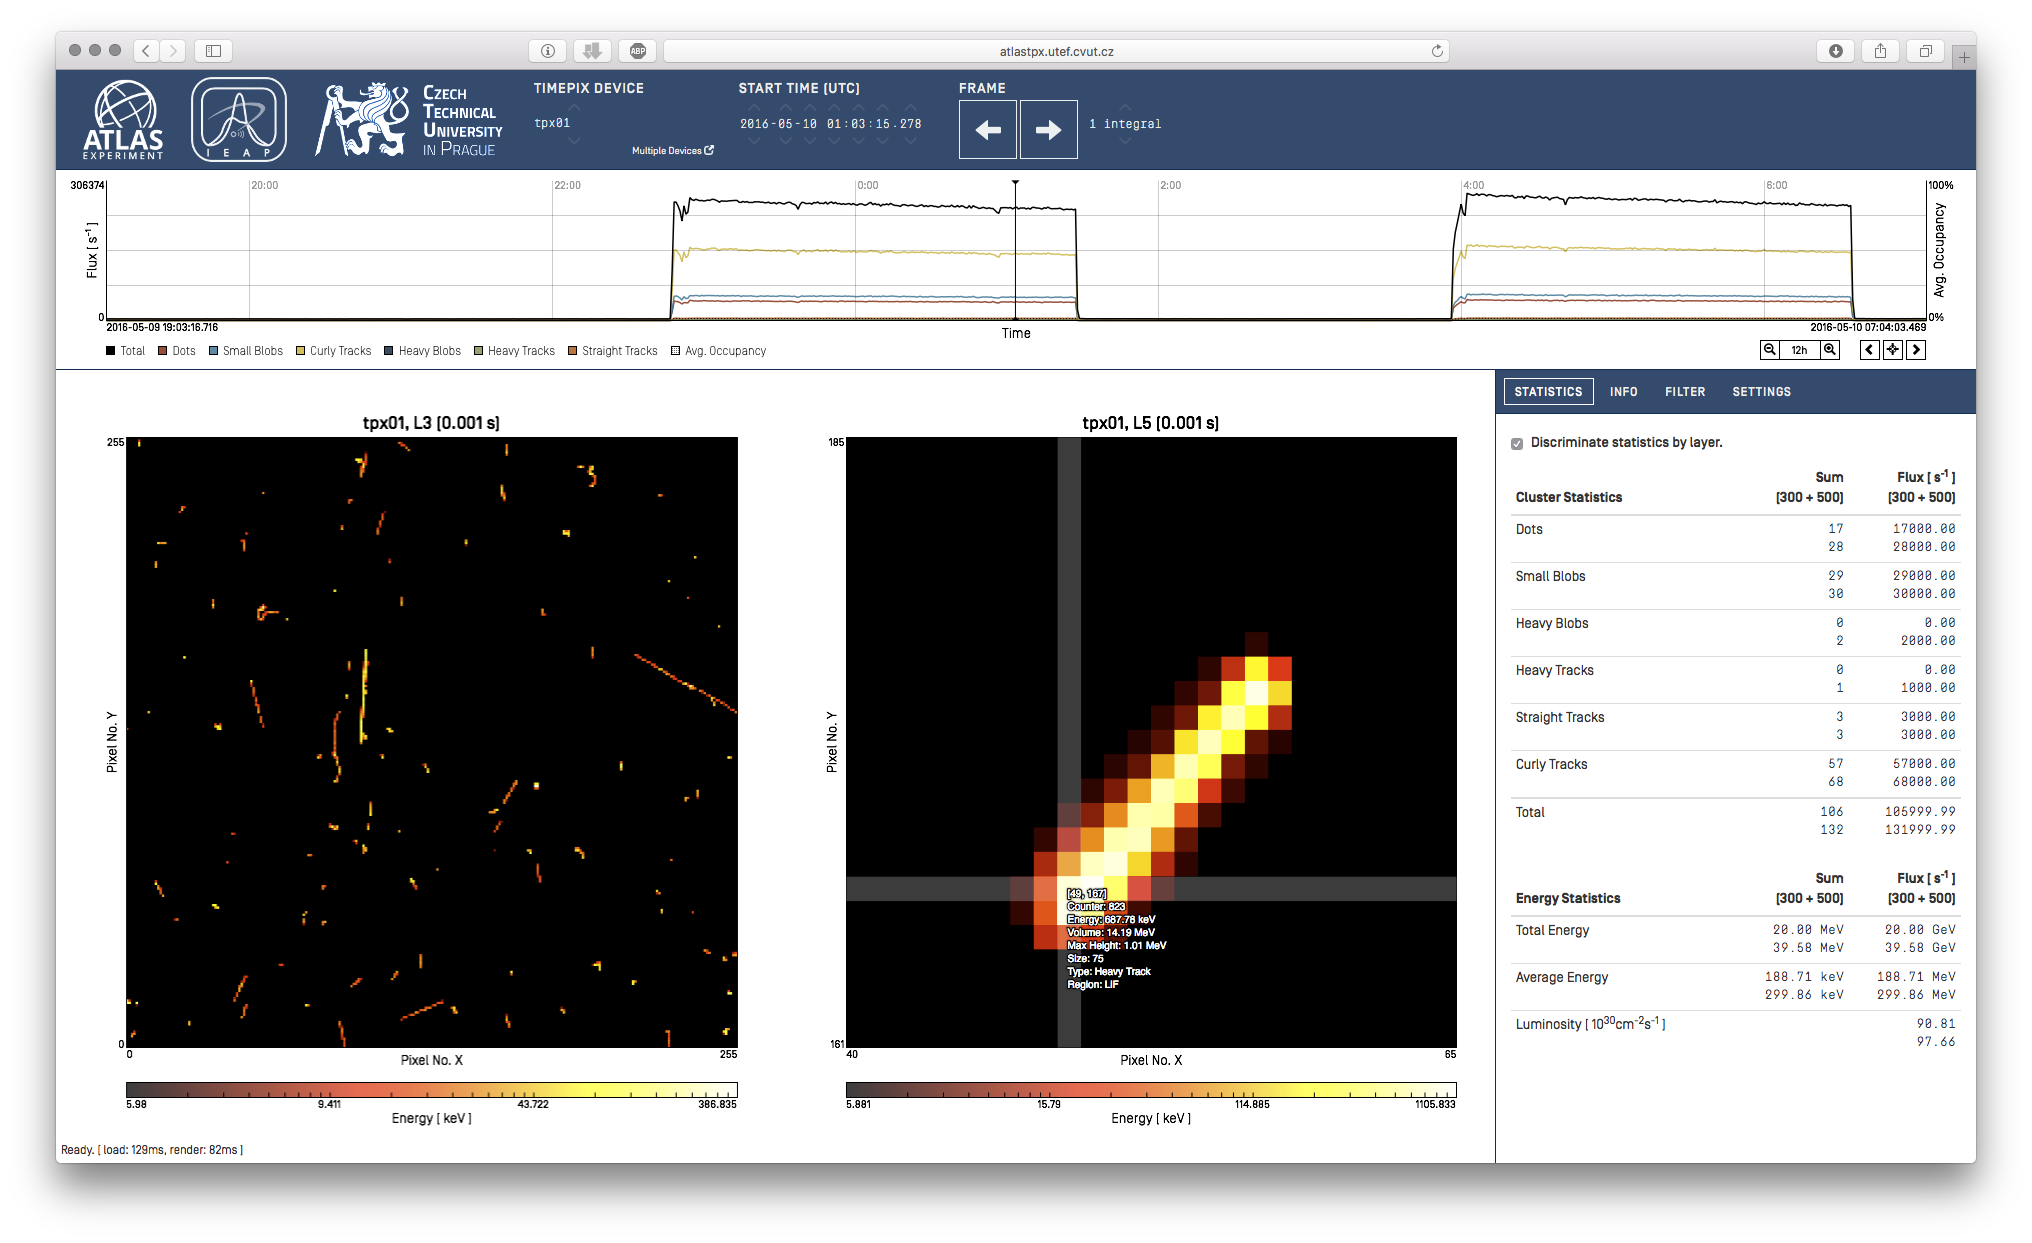
\includegraphics[width=\textwidth]{figures/screen-tpx01-crosshair-zoomed}
	\caption{Visualization with magnification enabled.}
	\label{fig:screenshot-zoomed}
	\end{subfigure}
\caption{Screenshots of the visualization UI.}
\label{fig:screenshots}
\end{center}
\end{figure}
